\documentclass[11pt, a4paper]{article}
\newcommand{\HomeworkHeader}{L00\_03-L01\_02}
% Shared LaTeX preamble for homework/*/main.tex

% --- Base layout ---
\usepackage[a4paper, top=2.5cm, bottom=2.5cm, left=2cm, right=2cm]{geometry}
\usepackage{fontspec}
\usepackage{xeCJK} % CJK fallback to avoid missing glyphs in Latin fonts
\usepackage{amsmath, amssymb, amsthm}
\usepackage{mathtools}
\usepackage{fancyhdr}
\usepackage{lastpage}
\usepackage[svgnames]{xcolor}
\usepackage{tikz}
\usetikzlibrary{automata, positioning, arrows.meta, bending, backgrounds}
\usepackage{pgfplots}
\pgfplotsset{compat=1.18}
\usepackage[most]{tcolorbox}
\usepackage{enumitem}

% --- Languages & fonts ---
\usepackage[english]{babel}
\babelprovide[import, main]{chinese}

\babelfont{rm}[UprightFont=*, BoldFont=* Bold, ItalicFont=* Italic, Scale=1.05]{Linux Libertine O}
\babelfont{sf}[UprightFont=*, BoldFont=* Bold, Scale=1.05]{Linux Biolinum O}
\babelfont[chinese]{rm}[
    UprightFont=*-Regular,
    BoldFont=*-Bold,
    ItalicFont=*-Regular,
    BoldItalicFont=*-Bold
]{Noto Serif CJK SC}
\babelfont[chinese]{sf}[
    UprightFont=*-Regular,
    BoldFont=*-Bold
]{Noto Sans CJK SC}
\babelfont{tt}{Noto Sans Mono}
\babelfont[chinese]{tt}{Noto Sans Mono CJK SC}

% xeCJK font setup (kept consistent with babelfont)
\setCJKmainfont{Noto Serif CJK SC}
\setCJKsansfont{Noto Sans CJK SC}
\setCJKmonofont{Noto Sans Mono CJK SC}

% --- Colors ---
\definecolor{primaryColor}{RGB}{46, 52, 64}
\definecolor{accentColor}{RGB}{94, 129, 172}
\definecolor{boxFill}{RGB}{236, 240, 241}
\definecolor{solLine}{RGB}{163, 190, 140}
\definecolor{expandColor}{RGB}{191, 97, 106}

% --- TikZ styles (DFA / NFA / PDA) ---
\tikzset{
    dfa_state/.style={
        state,
        thick,
        draw=accentColor,
        fill=boxFill,
        text=primaryColor,
        minimum size=1.1cm
    },
    dfa_edge/.style={
        ->,
        >=stealth,
        thick,
        draw=primaryColor,
        auto
    },
    pda_node/.style={
        state,
        thick,
        draw=accentColor,
        fill=boxFill,
        text=primaryColor,
        minimum size=1.2cm
    },
    pda_edge/.style={
        ->,
        >=stealth,
        thick,
        draw=primaryColor,
        auto
    },
    rule_expand/.style={
        pda_edge,
        draw=expandColor,
        text=expandColor
    },
    rule_match/.style={
        pda_edge,
        draw=solLine,
        text=solLine!80!black
    }
}

% --- Header / footer ---
\pagestyle{fancy}
\fancyhf{}
\lhead{\color{accentColor}\textbf{形式语言与自动机作业}}
\rhead{\color{primaryColor}\textbf{\HomeworkHeader}}
\cfoot{\small 第 \thepage \ 页,共 \pageref{LastPage} 页}
\setlength{\headheight}{24pt}
\addtolength{\topmargin}{-12pt}
\setlength{\emergencystretch}{2em}
\renewcommand{\headrulewidth}{0.4pt}
\renewcommand{\headrule}{\hbox to\headwidth{\color{accentColor}\leaders\hrule height \headrulewidth\hfill}}

% --- Problem box ---
\newtcolorbox[auto counter]{problem}[1][]{
    enhanced,
    breakable,
    colback=boxFill,
    colframe=accentColor,
    coltitle=white,
    fonttitle=\bfseries\large,
    title={题目 ~\thetcbcounter \quad #1},
    boxrule=0.5mm,
    arc=3mm,
    drop shadow=black!15!white,
    attach boxed title to top left={xshift=0.5cm, yshift*=-3mm},
    boxed title style={colback=accentColor}
}

% --- Solution environment ---
\newenvironment{solution}{
    \par\vspace{10pt}
    \noindent\textbf{\color{solLine} \Large \textit{Solution.}} \par
    \begingroup\color{primaryColor}\sloppy
    \leftskip1em \rightskip1em
    \noindent\rule{\textwidth}{0.4pt}
    \par\vspace{5pt}
}{
    \par\vspace{10pt}
    \noindent\rule[0.5ex]{\textwidth}{0.1pt}
    \endgroup
    \vspace{1.2cm}
}

% --- Title ---
\newcommand{\makeCustomTitle}[1]{
    \begin{center}
        \vspace*{1cm}
        {\Huge \bfseries \color{primaryColor} 作业 #1}\\
        \vspace{0.5cm}
        {\Large \color{accentColor} \today}
        \vspace{1.2cm}
    \end{center}
}


\begin{document}

\makeCustomTitle{L0.3 - L1.2:证明与 DFA}

\section*{L0.3:证明题}

% --- 题目 1 ---
\begin{problem}
试证明:每个包含两个或两个以上结点的图应包含有相等度数的两个结点。
\end{problem}

\begin{solution}
设图 $G$ 有 $n\ge 2$ 个结点。每个结点的度数属于集合 $\{0,1,2,\dots,n-1\}$。

注意不可能同时存在度数为 $0$ 的结点与度数为 $n-1$ 的结点:若某结点度为 $n-1$,它与所有其他结点相邻,则不存在孤立结点(度为 $0$)。

因此,$n$ 个结点的度数只能取自 $\{0,1,\dots,n-2\}$ 或 $\{1,2,\dots,n-1\}$,无论哪种情况都只有 $n-1$ 种可能取值。由抽屉原理(鸽巢原理),$n$ 个结点中必有两个结点度数相同。
\end{solution}

% --- 题目 2 ---
\begin{problem}
用反证法证明:素数有无穷多个。
\end{problem}

\begin{solution}
反证。假设素数只有有限多个,记为 $p_1,p_2,\dots,p_k$。考虑数
\[
N=p_1p_2\cdots p_k + 1.
\]
对任意 $i$,$N$ 除以 $p_i$ 余 $1$,因此没有任何 $p_i$ 能整除 $N$。于是 $N$ 要么本身是素数(与“素数只有 $k$ 个”矛盾),要么有某个素因子 $q$,但 $q$ 不在 $\{p_1,\dots,p_k\}$ 中(同样矛盾)。故假设不成立,素数有无穷多个。
\end{solution}

% --- 题目 3 ---
\begin{problem}
设 $S_n=1+2+\cdots+n$ 为前 $n$ 个自然数之和,$C_n=1^3+2^3+\cdots+n^3$ 为前 $n$ 个立方数之和。通过对 $n$ 的归纳证明下列等式,从而证明 $C_n=S_n^2$。
\[
S_n=\frac{n(n+1)}{2},\qquad C_n=\left(\frac{n(n+1)}{2}\right)^2.
\]
\end{problem}

\begin{solution}
\textbf{(1) 证明 $S_n=\frac{n(n+1)}{2}$。}

当 $n=1$ 时,$S_1=1=\frac{1\cdot 2}{2}$ 成立。假设对某个 $n$ 成立,即 $S_n=\frac{n(n+1)}{2}$。则
\[
S_{n+1}=S_n+(n+1)=\frac{n(n+1)}{2}+(n+1)=\frac{(n+1)(n+2)}{2},
\]
故对 $n+1$ 也成立,从而对所有 $n\in\mathbb{N}$ 成立。

\textbf{(2) 证明 $C_n=\left(\frac{n(n+1)}{2}\right)^2$。}

当 $n=1$ 时,$C_1=1^3=1=\left(\frac{1\cdot 2}{2}\right)^2$ 成立。假设对某个 $n$ 成立:
\[
C_n=\left(\frac{n(n+1)}{2}\right)^2.
\]
则
\[
\begin{aligned}
C_{n+1}
&=C_n+(n+1)^3\\
&=\left(\frac{n(n+1)}{2}\right)^2+(n+1)^3\\
&=(n+1)^2\left(\frac{n^2}{4}+n+1\right)
=(n+1)^2\cdot \frac{(n+2)^2}{4}
=\left(\frac{(n+1)(n+2)}{2}\right)^2.
\end{aligned}
\]
故对 $n+1$ 成立,从而对所有 $n$ 成立。由 $S_n=\frac{n(n+1)}{2}$ 得
\[
C_n=\left(\frac{n(n+1)}{2}\right)^2=S_n^2.
\]
\end{solution}

\section*{L1.1:DFA 基础}

% --- 题目 4 ---
\begin{problem}
下图给出了两台 DFA $M_1$ 和 $M_2$ 的状态图。回答下述关于这两台机器的问题:
\begin{enumerate}[label=(\alph*)]
    \item 它们的起始状态是什么?它们的接受状态集是什么?
    \item 对输入 \texttt{aabb},它们经过的状态序列是什么?
    \item 它们接受字符串 \texttt{aabb} 吗?
    \item 它们接受字符串 $\epsilon$ 吗?
\end{enumerate}
\end{problem}

\begin{solution}
\textbf{(a)} 从状态图上的入箭头可见,两台机器起始状态均为 $q_1$。

接受状态为双圈状态:
\[
F_1=\{q_2\},\qquad F_2=\{q_1,q_4\}.
\]

\textbf{(b)} 对输入 \texttt{aabb}:
\begin{itemize}
    \item $M_1$:$q_1 \xrightarrow{a} q_2 \xrightarrow{a} q_3 \xrightarrow{b} q_1 \xrightarrow{b} q_1$。
    \item $M_2$:$q_1 \xrightarrow{a} q_1 \xrightarrow{a} q_1 \xrightarrow{b} q_2 \xrightarrow{b} q_4$。
\end{itemize}

\textbf{(c)} $M_1$ 最终停在 $q_1\notin F_1$,因此不接受 \texttt{aabb};$M_2$ 最终停在 $q_4\in F_2$,因此接受 \texttt{aabb}。

\textbf{(d)} $\epsilon$ 时机器停在起始状态 $q_1$。因此 $M_1$ 不接受 $\epsilon$($q_1\notin F_1$),而 $M_2$ 接受 $\epsilon$($q_1\in F_2$)。
\end{solution}

% --- 题目 5 ---
\begin{problem}
DFA $M$ 的形式化描述为 $(\{q_1,q_2,q_3,q_4,q_5\},\{u,d\},\delta,q_3,\{q_3\})$,其中 $\delta$ 由下表给出。试画出这台机器的状态图。

\begin{center}
\begin{tabular}{c|cc}
 & $u$ & $d$ \\
\hline
$q_1$ & $q_1$ & $q_2$ \\
$q_2$ & $q_1$ & $q_3$ \\
$q_3$ & $q_2$ & $q_4$ \\
$q_4$ & $q_3$ & $q_5$ \\
$q_5$ & $q_4$ & $q_5$ \\
\end{tabular}
\end{center}
\end{problem}

\begin{solution}
\begin{center}
\begin{tikzpicture}[node distance=2.8cm]
    \node[dfa_state, initial, accepting] (q3) {$q_3$};
    \node[dfa_state, right of=q3] (q4) {$q_4$};
    \node[dfa_state, right of=q4] (q5) {$q_5$};
    \node[dfa_state, left of=q3] (q2) {$q_2$};
    \node[dfa_state, left of=q2] (q1) {$q_1$};

    \draw[dfa_edge]
        (q1) edge[loop above] node {$u$} (q1)
        (q1) edge[bend left=18] node {$d$} (q2)
        (q2) edge[bend left=18] node {$u$} (q1)
        (q2) edge[bend left=18] node {$d$} (q3)
        (q3) edge[bend left=18] node {$u$} (q2)
        (q3) edge[bend left=18] node {$d$} (q4)
        (q4) edge[bend left=18] node {$u$} (q3)
        (q4) edge[bend left=18] node {$d$} (q5)
        (q5) edge[loop above] node {$d$} (q5)
        (q5) edge[bend left=18] node {$u$} (q4);
\end{tikzpicture}
\end{center}

初态为 $q_3$,接受态为 $\{q_3\}$。
\end{solution}

% --- 题目 6 ---
\begin{problem}
画出识别下述语言的 DFA 状态图(字母表均为 $\{0,1\}$):
\begin{enumerate}[label=(\alph*)]
    \item $\{w \mid w \text{ 从 }1\text{ 开始且以 }0\text{ 结束}\}$
    \item $\{w \mid w \text{ 含有至少 3 个 }1\}$
    \item $\{w \mid w \text{ 含有子串 }0101\}$
    \item $\{w \mid |w|\ge 3\ \text{且第 3 个符号为 }0\}$
    \item $\{w \mid w \text{ 的奇数位置均为 }1\}$
\end{enumerate}
\end{problem}

\begin{solution}
\textbf{(a) 从 1 开始且以 0 结束}
\begin{center}
\begin{tikzpicture}[node distance=2.6cm]
    \node[dfa_state, initial] (s) {$s$};
    \node[dfa_state, right of=s] (q1) {$q_{1}$};
    \node[dfa_state, accepting, right of=q1] (q0) {$q_{0}$};
    \node[dfa_state, below of=q1] (dead) {$\bot$};

    \draw[dfa_edge]
        (s) edge node {$1$} (q1)
        (s) edge node [left] {$0$} (dead)
        (q1) edge[loop above] node {$1$} (q1)
        (q1) edge node {$0$} (q0)
        (q0) edge[bend left=18] node {$1$} (q1)
        (q0) edge[loop above] node {$0$} (q0)
        (dead) edge[loop left] node {$0,1$} (dead);
\end{tikzpicture}
\end{center}

\textbf{(b) 至少 3 个 1}
\begin{center}
\begin{tikzpicture}[node distance=2.3cm]
    \node[dfa_state, initial] (q0) {$0$};
    \node[dfa_state, right of=q0] (q1) {$1$};
    \node[dfa_state, right of=q1] (q2) {$2$};
    \node[dfa_state, accepting, right of=q2] (q3) {$\ge 3$};

    \draw[dfa_edge]
        (q0) edge[loop above] node {$0$} (q0)
        (q0) edge node {$1$} (q1)
        (q1) edge[loop above] node {$0$} (q1)
        (q1) edge node {$1$} (q2)
        (q2) edge[loop above] node {$0$} (q2)
        (q2) edge node {$1$} (q3)
        (q3) edge[loop above] node {$0,1$} (q3);
\end{tikzpicture}
\end{center}

\textbf{(c) 含有子串 0101}
\begin{center}
\begin{tikzpicture}[node distance=2.3cm]
    \node[dfa_state, initial] (p0) {$p_0$};
    \node[dfa_state, right of=p0] (p1) {$p_1$};
    \node[dfa_state, right of=p1] (p2) {$p_2$};
    \node[dfa_state, right of=p2] (p3) {$p_3$};
    \node[dfa_state, accepting, right of=p3] (p4) {$p_4$};

    \draw[dfa_edge]
        (p0) edge[loop above] node {$1$} (p0)
        (p0) edge node {$0$} (p1)
        (p1) edge[loop above] node {$0$} (p1)
        (p1) edge node {$1$} (p2)
        (p2) edge[bend left=18] node {$0$} (p3)
        (p2) edge[bend left=18] node [above] {$1$} (p0)
        (p3) edge[bend left=18] node {$1$} (p4)
        (p3) edge[bend left=18] node [below] {$0$} (p1)
        (p4) edge[loop above] node {$0,1$} (p4);
\end{tikzpicture}
\end{center}

\textbf{(d) 长度不小于 3 且第 3 个符号为 0}
\begin{center}
\begin{tikzpicture}[node distance=2.6cm]
    \node[dfa_state, initial] (r0) {$r_0$};
    \node[dfa_state, right of=r0] (r1) {$r_1$};
    \node[dfa_state, right of=r1] (r2) {$r_2$};
    \node[dfa_state, accepting, right of=r2] (acc) {$\checkmark$};
    \node[dfa_state, below of=r2] (dead) {$\bot$};

    \draw[dfa_edge]
        (r0) edge node {$0,1$} (r1)
        (r1) edge node {$0,1$} (r2)
        (r2) edge node {$0$} (acc)
        (r2) edge node [right] {$1$} (dead)
        (acc) edge[loop above] node {$0,1$} (acc)
        (dead) edge[loop right] node {$0,1$} (dead);
\end{tikzpicture}
\end{center}

\textbf{(e) 奇数位置均为 1}
\begin{center}
\begin{tikzpicture}[node distance=2.6cm]
    \node[dfa_state, initial, accepting] (odd) {$O$};
    \node[dfa_state, accepting, right of=odd] (even) {$E$};
    \node[dfa_state, below of=even] (dead) {$\bot$};

    \draw[dfa_edge]
        (odd) edge node {$1$} (even)
        (odd) edge node [left] {$0$} (dead)
        (even) edge[bend left=18] node {$0,1$} (odd)
        (dead) edge[loop right] node {$0,1$} (dead);
\end{tikzpicture}
\end{center}
其中 $O$ 表示“下一位是奇数位置”,$E$ 表示“下一位是偶数位置”。空串 $\epsilon$ 在 $O$ 上直接接受。
\end{solution}

\section*{L1.2:DFA 构造(交 / 补)}

% --- 题目 7 ---
\begin{problem}
下面每个语言都是两个简单语言的交。构造识别这些语言的 DFA(字母表为 $\{a,b\}$):
\begin{enumerate}[label=(\alph*)]
    \item $\{w \mid w \text{ 含有至少 3 个 } a \text{ 和至少 2 个 } b\}$
    \item $\{w \mid w \text{ 含有偶数个 } a \text{ 且含有 1 个或 2 个 } b\}$
    \item $\{w \mid w \text{ 从 } a \text{ 开始并且最多有 1 个 } b\}$
    \item $\{w \mid w \text{ 含有奇数个 } a \text{ 并且以 } b \text{ 结束}\}$
    \item $\{w \mid |w| \text{ 为偶数并且有奇数个 } a\}$
\end{enumerate}
\end{problem}

\begin{solution}
以下给出“状态含义 + 转移表”的构造(均为饱和计数/直积构造,直接可画成状态图)。

\textbf{(a) 至少 3 个 $a$ 且至少 2 个 $b$}

取状态集合 $Q=\{0,1,2,3\}\times\{0,1,2\}$,第一维记录 $a$ 的个数($3$ 表示 $\ge 3$),第二维记录 $b$ 的个数($2$ 表示 $\ge 2$)。初态 $(0,0)$,接受态 $F=\{(3,2)\}$。转移为饱和加一:
\[
\delta\big((i,j),a\big)=\big(\min(i+1,3),\,j\big),\qquad
\delta\big((i,j),b\big)=\big(i,\,\min(j+1,2)\big).
\]

\textbf{(b) 偶数个 $a$ 且 $b$ 的个数为 1 或 2}

取状态为 $(p,k)$,其中 $p\in\{E,O\}$ 表示 $a$ 的奇偶性,$k\in\{0,1,2,\ge 3\}$ 表示 $b$ 的个数($\ge 3$ 为陷阱态)。初态 $(E,0)$,接受态 $F=\{(E,1),(E,2)\}$。转移表:
\begin{center}
\begin{tabular}{c|cc}
状态 & $a$ & $b$ \\
\hline
$(E,0)$ & $(O,0)$ & $(E,1)$ \\
$(O,0)$ & $(E,0)$ & $(O,1)$ \\
$(E,1)$ & $(O,1)$ & $(E,2)$ \\
$(O,1)$ & $(E,1)$ & $(O,2)$ \\
$(E,2)$ & $(O,2)$ & $(E,\ge 3)$ \\
$(O,2)$ & $(E,2)$ & $(O,\ge 3)$ \\
$(E,\ge 3)$ & $(O,\ge 3)$ & $(E,\ge 3)$ \\
$(O,\ge 3)$ & $(E,\ge 3)$ & $(O,\ge 3)$ \\
\end{tabular}
\end{center}

\textbf{(c) 从 $a$ 开始且最多 1 个 $b$}

状态集合 $\{s, A_0, A_1, \bot\}$,$s$ 表示尚未读入符号;$A_0$ 表示已以 $a$ 开始且目前 $b$ 个数为 0;$A_1$ 表示已以 $a$ 开始且目前 $b$ 个数为 1;$\bot$ 为陷阱态。初态 $s$,接受态 $F=\{A_0,A_1\}$。转移表:
\begin{center}
\begin{tabular}{c|cc}
状态 & $a$ & $b$ \\
\hline
$s$ & $A_0$ & $\bot$ \\
$A_0$ & $A_0$ & $A_1$ \\
$A_1$ & $A_1$ & $\bot$ \\
$\bot$ & $\bot$ & $\bot$ \\
\end{tabular}
\end{center}

\textbf{(d) 奇数个 $a$ 且以 $b$ 结束}

状态表示 $(p,\ell)$:$p\in\{E,O\}$ 为 $a$ 的奇偶性,$\ell\in\{\#,a,b\}$ 为“最后读到的符号”($\#$ 表示空)。初态 $(E,\#)$,接受态 $F=\{(O,b)\}$。转移规则:
\[
\delta((p,\ell),a)=(\overline{p},a),\qquad \delta((p,\ell),b)=(p,b),
\]
其中 $\overline{E}=O,\ \overline{O}=E$。

\textbf{(e) 长度为偶数且 $a$ 的个数为奇数}

状态表示 $(L,P)$:$L\in\{E,O\}$ 表示长度奇偶性,$P\in\{E,O\}$ 表示 $a$ 的奇偶性。初态 $(E,E)$,接受态 $F=\{(E,O)\}$。转移:
\[
\delta((L,P),a)=(\overline{L},\overline{P}),\qquad
\delta((L,P),b)=(\overline{L},P).
\]
\end{solution}

% --- 题目 8 ---
\begin{problem}
下述每个语言都是一个简单语言的补。构造识别这些语言的 DFA(字母表为 $\{a,b\}$):
\begin{enumerate}[label=(\alph*)]
    \item $\{w \mid w \text{ 不含子串 }ab\}$
    \item $\{w \mid w \text{ 中既不含子串 }ab \text{ 也不含子串 }ba\}$
    \item $\{w \mid w \text{ 是不在 } a^*b^* \text{ 中的任意串}\}$
    \item $\{w \mid w \text{ 是恰好不含 2 个 }a\text{ 的任意串}\}$
\end{enumerate}
\end{problem}

\begin{solution}
\textbf{(a) 不含子串 $ab$}

状态集合 $\{q_0,q_1,\bot\}$:$q_0$ 表示“当前未处于刚读到 $a$ 的状态”(安全),$q_1$ 表示“最后一个符号是 $a$”(若再读 $b$ 就违例),$\bot$ 为已出现 $ab$。初态 $q_0$,接受态 $F=\{q_0,q_1\}$。转移表:
\begin{center}
\begin{tabular}{c|cc}
状态 & $a$ & $b$ \\
\hline
$q_0$ & $q_1$ & $q_0$ \\
$q_1$ & $q_1$ & $\bot$ \\
$\bot$ & $\bot$ & $\bot$ \\
\end{tabular}
\end{center}

\textbf{(b) 既不含 $ab$ 也不含 $ba$}

该语言等价于“全是 $a$ 的串”或“全是 $b$ 的串”(以及空串)。状态集合 $\{s,A,B,\bot\}$,初态 $s$,接受态 $F=\{s,A,B\}$。转移表:
\begin{center}
\begin{tabular}{c|cc}
状态 & $a$ & $b$ \\
\hline
$s$ & $A$ & $B$ \\
$A$ & $A$ & $\bot$ \\
$B$ & $\bot$ & $B$ \\
$\bot$ & $\bot$ & $\bot$ \\
\end{tabular}
\end{center}

\textbf{(c) 不在 $a^*b^*$ 中}

一个串不在 $a^*b^*$ 中当且仅当出现过某个位置先读到 $b$,之后又读到 $a$(即包含子串 $ba$)。状态集合 $\{q_0,q_1,q_{\checkmark}\}$:$q_0$ 表示尚未见到 $b$;$q_1$ 表示已经进入 $b^*$ 阶段(见过 $b$);$q_{\checkmark}$ 表示已出现 $ba$。初态 $q_0$,接受态 $F=\{q_{\checkmark}\}$。转移表:
\begin{center}
\begin{tabular}{c|cc}
状态 & $a$ & $b$ \\
\hline
$q_0$ & $q_0$ & $q_1$ \\
$q_1$ & $q_{\checkmark}$ & $q_1$ \\
$q_{\checkmark}$ & $q_{\checkmark}$ & $q_{\checkmark}$ \\
\end{tabular}
\end{center}

\textbf{(d) 恰好不含 2 个 $a$}

即接受所有 $a$ 的个数不等于 $2$ 的串。取状态 $\{0,1,2,\ge 3\}$ 记录 $a$ 的个数($\ge 3$ 饱和),初态 $0$,接受态 $F=\{0,1,\ge 3\}$(唯一拒绝态为 $2$)。转移:
\[
\delta(k,b)=k,\qquad
\delta(k,a)=\min(k+1,3).
\]
\end{solution}

\end{document}
